%!TEX root=./LIVRO.tex

\chapter[Simulado 3]{Simulado}

\num{1} Leia os textos.

\begin{myquote}
\textbf{TEXTO I}

É PROHIBIDO COLLOCAR CARTAZES E ANNUNCIOS EM TODO O EDIFICIO D'ESTA ORDEM.
\end{myquote}

\begin{myquote}
\textbf{TEXTO II}

É PROIBIDO COLOCAR CARTAZES E ANÚNCIOS EM TODO O EDIFÍCIO.
\end{myquote}

O texto II é uma reescrita do texto I, e ambos representam estágios
diferentes da língua portuguesa. Nesse sentido, exemplificam a variação
linguística

\begin{multicols}{2}
\begin{escolha}
\item
  social.
\item
  regional.
\item
  histórica.
\item
  situacional.
\end{escolha}
\end{multicols}

\num{2} Leia a fábula.

\begin{myquote}
\textbf{A raposa e as uvas}

Uma raposa, aproximando-se de uma parreira, viu que ela estava carregada
de uvas maduras e apetitosas. Com água na boca, desejou-as comer e, para
tanto, começou a fazer esforços para subir até elas. Porém, como
estivessem as uvas muito altas e fosse muito difícil a subida, a raposa
tentou, mas não conseguiu alcançá-las. Disse então:

--- Estas uvas estão muito azedas e podem desbotar os meus dentes; não
quero colhê-las agora porque não gosto de uvas que não estão maduras.

E, dito isso, se foi.

\fonte{Joseph Shafan. \textit{As fábulas de Esopo}. Disponível em:
http://www.dominiopublico.gov.br/download/texto/ea000378.pdf. Acesso em 28 set. 2023.}
\end{myquote}

No gênero narrativo fábula, normalmente se pode reconhecer um ditado
popular que expressa um ensinamento. Essa fábula se relaciona com qual ditado popular?

\begin{escolha}
\item Saco vazio não para em pé.

\item Quem tem pressa come cru.

\item Quem desdenha quer comprar.

\item Há males que vêm para o bem.
\end{escolha}

\num{3} Em uma campanha de doação de sangue, criou-se um anúncio em que, além da imagem de 
um cantor famoso, apareciam os dizeres reproduzidos a seguir.

\begin{center}
\begin{myquote}
\textbf{Doar sangue dói? Um pouquinho!}

Mas tem tanta coisa no dia a dia que dói mais e não salva vidas: depilação; treino pesado na academia; o 
visualizado e não respondido do crush; tatuar; segurar essa barra que é gostar de você.

\textbf{Deixe o medo de lado e seja solidário}
\end{myquote}
\end{center}


O recurso persuasivo utilizado na campanha é o efeito de humor, alcançado, sobretudo, por meio

\begin{escolha}
\item da relativização da dor.
\item da citação de uma canção.
\item da referência ao cotidiano.
\item da oposição medo-solidariedade.
\end{escolha}

\num{4} Leia o trecho de um poema.

\begin{myquote}
A criança que fui chora na estrada.\\
Deixei-a ali quando vim ser quem sou.\\
Mas hoje, vendo que o que sou é nada,\\
Quero ir buscar quem fui onde ficou.

\fonte{Fernando Pessoa. A criança que fui chora na estrada. http://arquivopessoa.net/textos/2455. Acesso em 28 setembro 2023.}
\end{myquote}

\pagebreak
Em razão do gênero literário a que pertence, o texto caracteriza-se por
colocar em foco

\begin{escolha}
\item os sentimentos subjetivos do eu lírico.

\item a clareza e a objetividade da mensagem.

\item a interpretação dramática de uma cena.

\item os elementos da sequência da narrativa.
\end{escolha}

\num{5} Documento que acompanha um medicamento para orientar o
usuário quanto à ingestão, a bula de remédio contém: indicações;
contraindicações; efeitos secundários; apresentação; fórmula ou composição;
nome do laboratório; posologia (dose adequada). O conteúdo 
da bula de remédio e sua finalidade comunicativa justificam,
na escrita desse gênero, o emprego de linguagem

\begin{escolha}
\item objetiva, para expor as informações do medicamento.

\item argumentativa, para dar uma opinião sobre o medicamento.

\item narrativa, para relatar as etapas de produção do medicamento.

\item figurada, para facilitar a compreensão dos dados do medicamento.
\end{escolha}


Texto para as questões de 6 a 8.

\begin{myquote}
A história do futebol é uma triste viagem do prazer ao dever. {[}...{]}
O jogo se transformou em espetáculo, com poucos protagonistas e muitos
espectadores, futebol para olhar, e o espetáculo se transformou num dos
negócios mais lucrativos do mundo, que não é organizado para ser jogado,
mas para impedir que se jogue. A tecnocracia do esporte profissional foi
impondo um futebol de pura velocidade e muita força, que renuncia à
alegria, atrofia a fantasia e proíbe a ousadia. Por sorte ainda aparece
nos campos {[}...{]} algum atrevido que sai do roteiro e comete o
disparate de driblar o time adversário inteirinho, além do juiz e do
público das arquibancadas {[}...{]}.

\fonte{E. Galeano. \emph{Futebol ao sol e à sombra}. Porto Alegre: L\&PM, 1995.
(Fragmento.)}
\end{myquote}

\pagebreak

\num{6} Nas relações de sentido construídas no texto, o termo ``dever'' se
relaciona, no contexto do futebol, com a ideia de roteiro, assim como
``prazer'' se relaciona com a ideia de

\begin{multicols}{2}
\begin{escolha}
\item improviso.

\item obrigação.

\item velocidade.

\item tecnocracia.
\end{escolha}
\end{multicols}

\num{7} Do ponto de vista do enunciador, o futebol do dever e o futebol do prazer
caracterizam-se, respectivamente, por

\begin{multicols}{2}
\begin{escolha}
\item arte e criatividade.

\item velocidade e força.

\item monotonia e divertimento.

\item profissionalismo e várzea.
\end{escolha}
\end{multicols}

\num{8} Para realçar as qualidades do futebol do prazer sobre as do futebol do
dever, o autor emprega exagero em

\begin{escolha}
\item ``o espetáculo se transformou num dos negócios mais lucrativos do
mundo.''

\item ``A tecnocracia do esporte profissional foi impondo um futebol de
pura velocidade e muita força.''

\item ``O jogo se transformou em espetáculo, com poucos protagonistas e muitos espectadores.''

\item ``comete o disparate de driblar o time adversário inteirinho, além do juiz e do público das arquibancadas.''
\end{escolha}

\num{9} Leia o texto.

\begin{myquote}
No Distrito Federal, uma reportagem revelou orientações ilegais contidas
em material utilizado no curso de formação de praças da PM. A Promotoria
Militar do Ministério Público do Distrito Federal e Territórios pediu
que a Corregedoria da Polícia Militar do DF abra investigação sobre a
denúncia, feita pelo colunista do UOL, Chico Alves.

Numa apresentação de PowerPoint sobre disciplina, ética, chefia e
liderança, conceitos teriam sido distorcidos para afirmar que, ao forjar
um flagrante ou praticar pequena tortura, o policial estaria agindo
corretamente.

\fonte{Disponível em:
\emph{https://agenciabrasil.ebc.com.br/direitos-humanos/noticia/2023-03/policia-militar-do-piaui-quer-formacao-antirracista-dos-agentes}.
Acesso em: 03 mar. 2023.}
\end{myquote}

\pagebreak

Em se tratando do gênero notícia, a forma verbal ``teriam sido
distorcidos'' demonstra a intenção de

\begin{escolha}
\item reforçar a denúncia, pois a distorção dos conceitos ficou comprovada.

\item duvidar da veracidade do fato, pois a instituição denunciada é de confiança.

\item atribuir a afirmação a um terceiro, pois a denúncia foi feita por outro jornal.

\item amenizar a gravidade do fato, pois a distorção respeitou os limites da lei.
\end{escolha}

\num{10} Para Marcos Bagno a afirmação de que o português é muito difícil,
muito dita principalmente por estudantes, é um mito. Trata-se de uma afirmação
falsa, porque só considera as regras da modalidade linguística aprendida na
escola, e não ao uso real que eles mesmos fazem da língua. Esse 
mito do português como língua difícil poderia ter surgido porque

\begin{escolha}
\item a escola ensina a gramática da língua de forma errada para os
estudantes.

\item os estudantes não se dedicam ao estudo da língua para aprenderem a
gramática.

\item a língua do cotidiano não tem regras, ao contrário da língua ensinada
na escola.

\item as pessoas pensam que a língua se limita às regras gramaticais ensinadas na escola.
\end{escolha}

\begin{figure}[H]
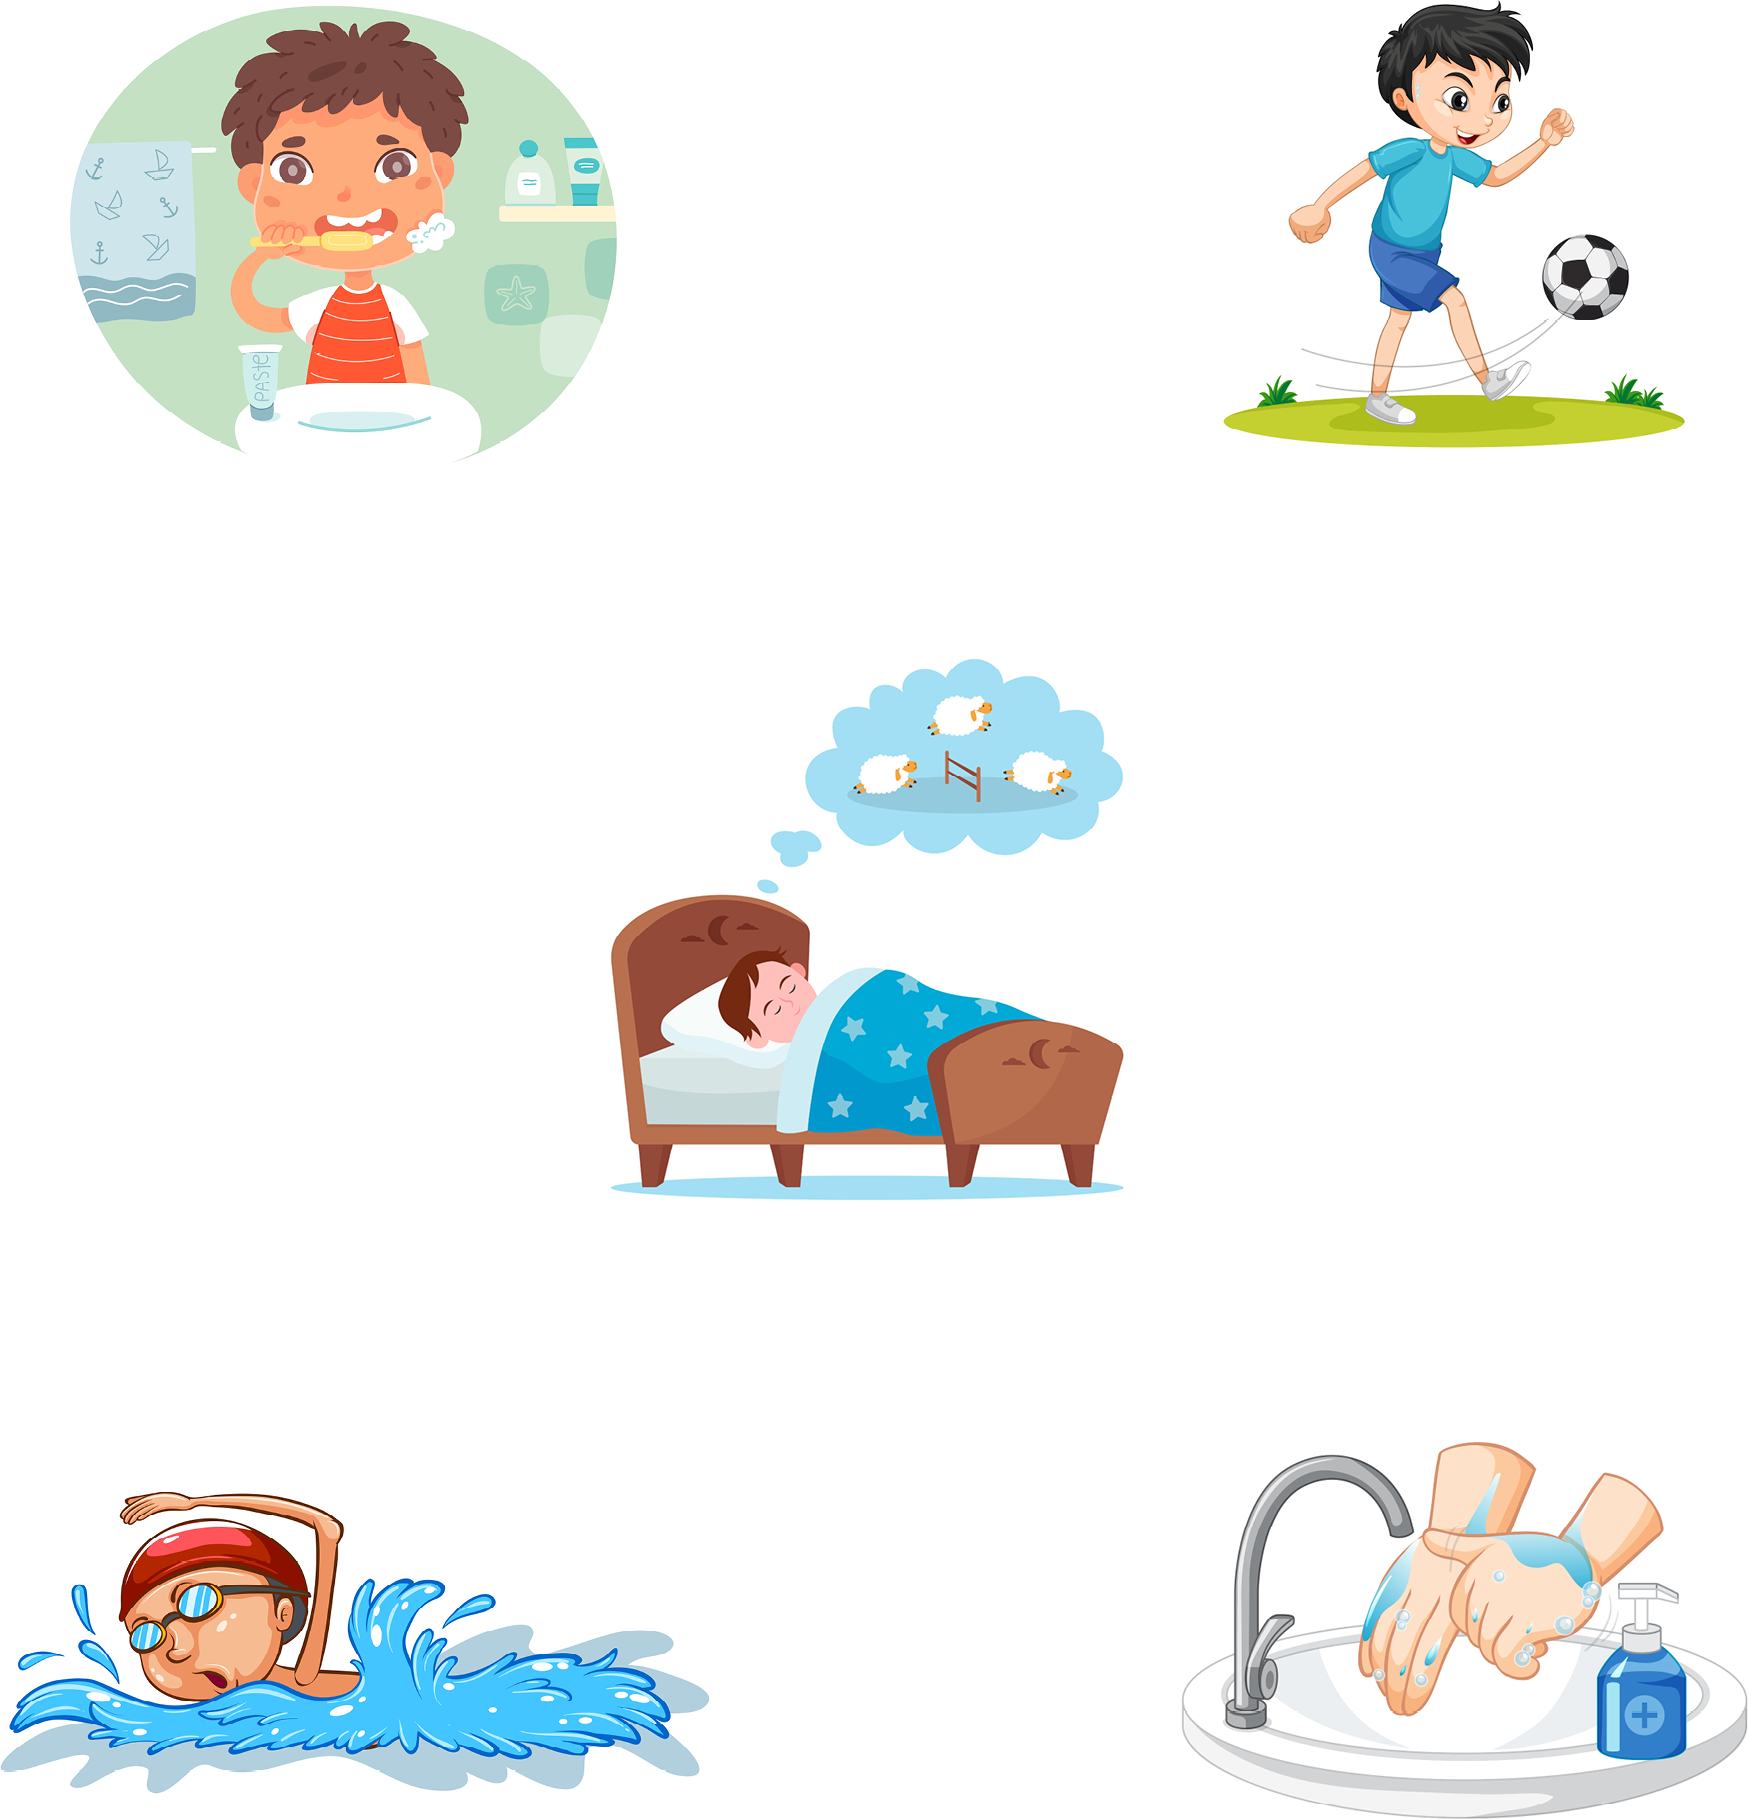
\includegraphics[width=\textwidth]{imgSAEB_8_POR/media/image57.png}
\end{figure}

\pagebreak

\num{11} Leia o texto.

\begin{myquote}
VERA -- (sentando-se pensativa) Algo de ruim aconteceu a ele. Pode até
estar morto! Oh, Michael, estou tão angustiada com Dmitri.

MICHAEL -- Nunca vai amar outra pessoa além dele?

VERA -- (sorrindo) Não sei. Há muitas outras coisas para fazer no mundo
além de amar.

MICHAEL -- Nada mais vale a pena, Vera.

PETER -- Que barulho é este, Vera? (ouve-se um ruído metálico)

VERA -- (levantando-se e indo até a porta) Não sei, pai. Não se parece
com sinos de gado, senão poderia ser Nicholas retornando da feira.

\fonte{Oscar Wilde. Tradução de Doris Goettems, da Editora Landmark, de 2011.}
\end{myquote}

O que caracteriza o texto como peça teatral é a presença de

\begin{escolha}
\item rubricas com instruções de interpretação da cena.

\item emoções subjetivas dos personagens, como a angústia.

\item indicações do tempo e espaço em que se passa a história.

\item discurso indireto em que as falas são reproduzidas pelo narrador.
\end{escolha}

\num{12} Leia o texto.

\begin{myquote}
A gente se acostuma a morar em apartamentos de fundos e a não ter outra
vista que não as janelas ao redor. E, porque não tem vista, logo se
acostuma a não olhar para fora. E, porque não olha para fora, logo se
acostuma a não abrir de todo as cortinas. E, porque não abre as
cortinas, logo se acostuma a acender mais cedo a luz. {[}...{]}

\fonte{Marina Colasanti. \emph{Eu sei, mas não devia}. Rio de Janeiro: Rocco,
1996. (Fragmento.)}
\end{myquote}

A repetição de certas palavras no texto contribui para a progressão textual ao

\begin{escolha}
\item narrar a rotina da autora, do começo ao fim do dia.

\item justificar a preferência da autora por morar numa casa.

\item descrever ações realizadas, na ordem em que ocorreram.

\item enumerar situações que são consequências umas das outras.
\end{escolha}

\pagebreak

\num{13} Leia o texto.

\begin{myquote}
\textbf{TÍTULO I}

\textbf{Dos Princípios Fundamentais}

\textbf{Art. 1º} A República Federativa do Brasil, formada pela união
indissolúvel dos Estados e Municípios e do Distrito Federal,
constitui-se em Estado Democrático de Direito e tem como fundamentos:

I --- a soberania;

II --- a cidadania; {[}...{]}

\textbf{Art. 2º} São Poderes da União, independentes e harmônicos entre si, o
Legislativo, o Executivo e o Judiciário.

\textbf{Art. 3º} Constituem objetivos fundamentais da República Federativa do
Brasil:

I --- construir uma sociedade livre, justa e solidária;

II --- garantir o desenvolvimento nacional; {[}...{]}

\fonte{Constituição da República Federativa do Brasil de 1988.}
\end{myquote}

O trecho transcrito da Constituição é exemplar do gênero lei, pois

\begin{escolha}
\item determina as obrigações a serem cumpridas pelos cidadãos.

\item apresenta um vocabulário conhecido apenas por advogados.

\item estrutura os assuntos em artigos, elemento básico do gênero.

\item narra a evolução do país até se tornar uma república federativa.
\end{escolha}

\begin{figure}[H]
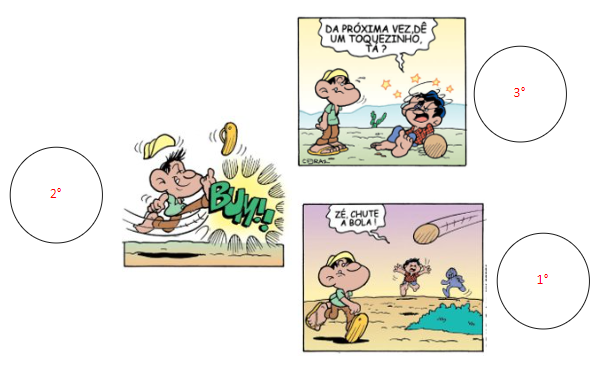
\includegraphics[width=\textwidth]{imgSAEB_8_POR/media/image58.png}
\end{figure}

Texto para as questões 14 e 15.

\begin{myquote}
Vivia longe dos homens, só se dava bem com animais. Os seus pés duros
quebravam espinhos e não sentiam a quentura da terra. Montado,
confundia-se com o cavalo, grudava-se a ele. E falava uma linguagem
cantada, monossilábica e gutural, que o companheiro entendia. A pé, não
se aguentava bem. Pendia para um lado, para o outro lado, cambaio, torto
e feio. Às vezes, utilizava nas relações com as pessoas a mesma língua
com que se dirigia aos brutos -- exclamações, onomatopeias. Na verdade
falava pouco. Admirava as palavras compridas e difíceis da gente da
cidade, tentava reproduzir algumas em vão, mas sabia que elas eram
inúteis e talvez perigosas.

\fonte{Graciliano Ramos. \textit{Vidas secas}. Rio de Janeiro: Record, 2013.}
\end{myquote}

\num{14} A descrição física e psicológica do personagem contribui caracterizá-lo
como alguém

\begin{escolha}
\item tolo.

\item rústico.

\item analfabeto.

\item mal-humorado.
\end{escolha}

\num{15} Em ``Na verdade falava pouco'', o narrador introduz uma

\begin{escolha}
\item conclusão.

\item reformulação.

\item exemplificação.

\item particularização.
\end{escolha}
